\tikzstyle{boxes}=[draw=black, rounded corners,very thick]
\begin{center}
{
%\fontfamily{roman}{\fontsize{10}{10}\selectfont

\begin{tikzpicture}[shorten >=1pt,draw=black!50, x = 1 in, y = 1 in,  node distance=20pt]
\draw[draw=none, use as bounding box](-0.5,-0.1) rectangle (3.5,2.85);
\node[anchor=north west,align = left, text width=9.5 cm] at (-0.5,2.85) {Sometimes, simple lists of atomic propties are sufficient, especially if informed by domain knowledge:};
\visible<1->{\node (fullc) at (2.15,0.70) {\includegraphics[width=4.5 cm]{representations/images/full}};}
%\draw[help lines,step=0.82] (0,0) grid (3.3,4);


%\node [anchor=north,rotate=90] (train) at (0.001,0.4) {nearest train.};

%\node [anchor=north,rotate=90] (train) at (0.001,1.2) {Fe(II)};
%\node [anchor=north,rotate=90] (train) at (0.87,1.2) {Fe(II)};
%\node [anchor=north,rotate=90] (train) at (1.69,1.2) {Fe(II)};



\visible<2->{\node [ text width = 2.5 cm, text badly centered,red] at (0.5-0.25,2.65-0.5) {\small metal properties}{};}
\visible<3->{\node [ text width = 3 cm, text badly centered,blue] at (1.6-0.25,2.65-0.5) {\small first coord. shell}{};}
\visible<4->{\node [ text width = 3 cm, text badly centered,darkgreen] at (2.7-0.25,2.65-0.5) {\small global properties}{};}
\visible<2->{\node [trapezium,trapezium left angle=70, trapezium right angle=110, draw, ultra thick, red, minimum size = 0.7in,rounded corners] at (0.5-0.25,2.10-0.4) {};}
\visible<3->{\node [trapezium,trapezium left angle=70, trapezium right angle=110, draw, ultra thick, blue, minimum size = 0.7in,rounded corners] at (1.6-0.25,2.10-0.4) {};}
\visible<4->{\node [trapezium,trapezium left angle=70, trapezium right angle=110, draw, ultra thick, darkgreen, minimum size = 0.7in,rounded corners] at (2.7-0.25,2.10-0.4) {};}



%\foreach \x in {0.525,1.05,2.15}
%	\draw [ultra thick,black] (\x,0)--(\x,1.64);




\visible<2->{\node []  (mid) at (0.58-0.25,2.30-0.4) {\small  identity};}
\visible<2->{\node []  (oxx) at (0.425-0.25,1.90-0.4) {\small oxidation state};}
\visible<2->{\node [firebrick]  (mettxt) at (0.50-0.25,2.1-0.4) {\bf{Fe(II)}};}

\visible<3->{\node [text width = 0.75in,text badly centered]  (mid) at (1.68-0.25,2.30-0.4) {\small };}
\visible<3->{\node []  (oxx) at (1.55-0.25,1.90-0.425) {\small $\max \Delta \chi$};}
\visible<3->{\node [orange]  (liex) at (1.6-0.25,2.10-0.4) {{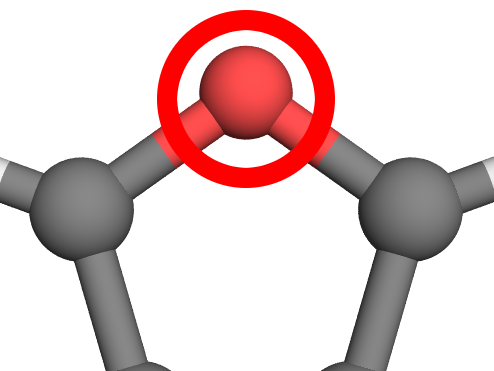
\includegraphics[width=0.4in]{representations/images/furanzoom}}};}
\visible<3->{\node [red]  (chiox) at (1.50-0.25,2.30-0.4) {\scriptsize $\chi = 3.44 $};}
\visible<3->{\node [gray,rectangle,fill=white,minimum height = 0.1cm,inner sep =0]  (chiC) at (1.75-0.25,2.0-0.4) {\scriptsize $\chi = 2.55 $};}

\visible<4->{\node[inner sep=0pt] (d3) at (2.68-0.25,2.18-0.4){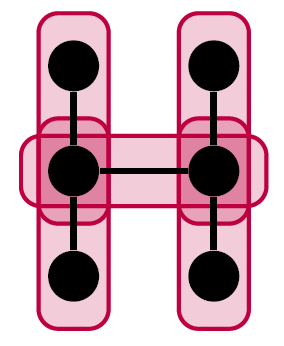
\includegraphics[width=0.4in,angle=90]{representations/images/desc3}};}
\visible<4->{\node []  (oxx) at (2.65-0.25,1.90-0.4) {\small Kier index};}



\visible<5->{\node [anchor=south west]  (liex) at (-0.5,-0.1) {{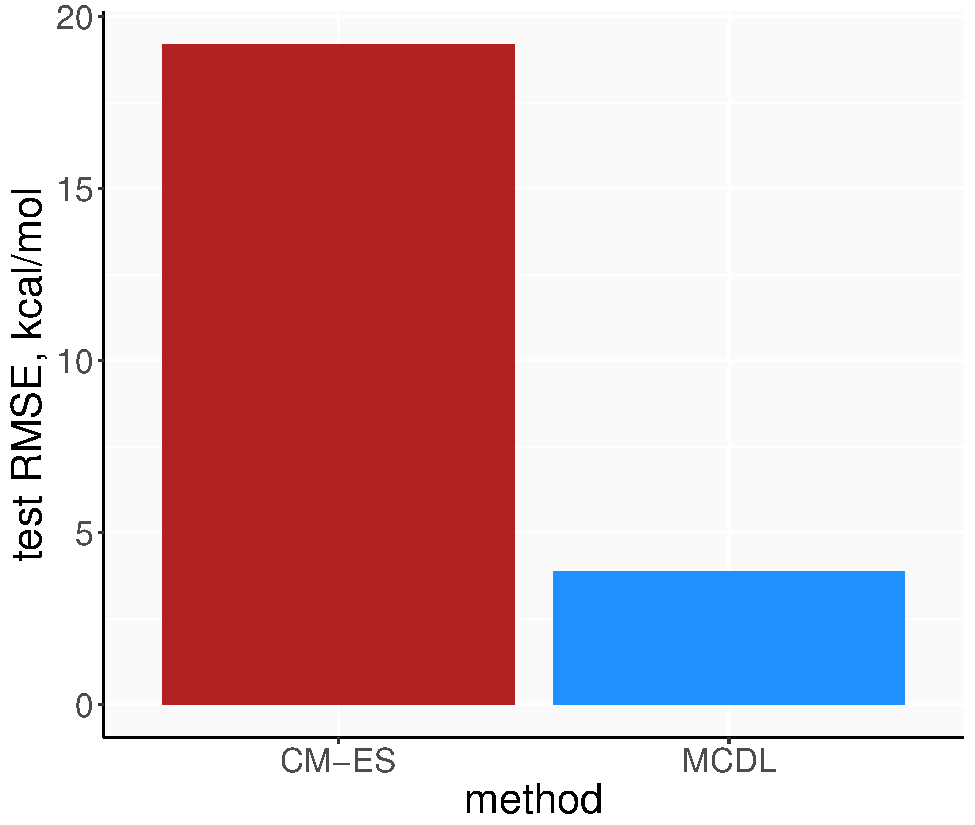
\includegraphics[width=4 cm]{representations/figures/error_comp}}};}


%\node [orange]  (liex) at (1.5,0.75) {{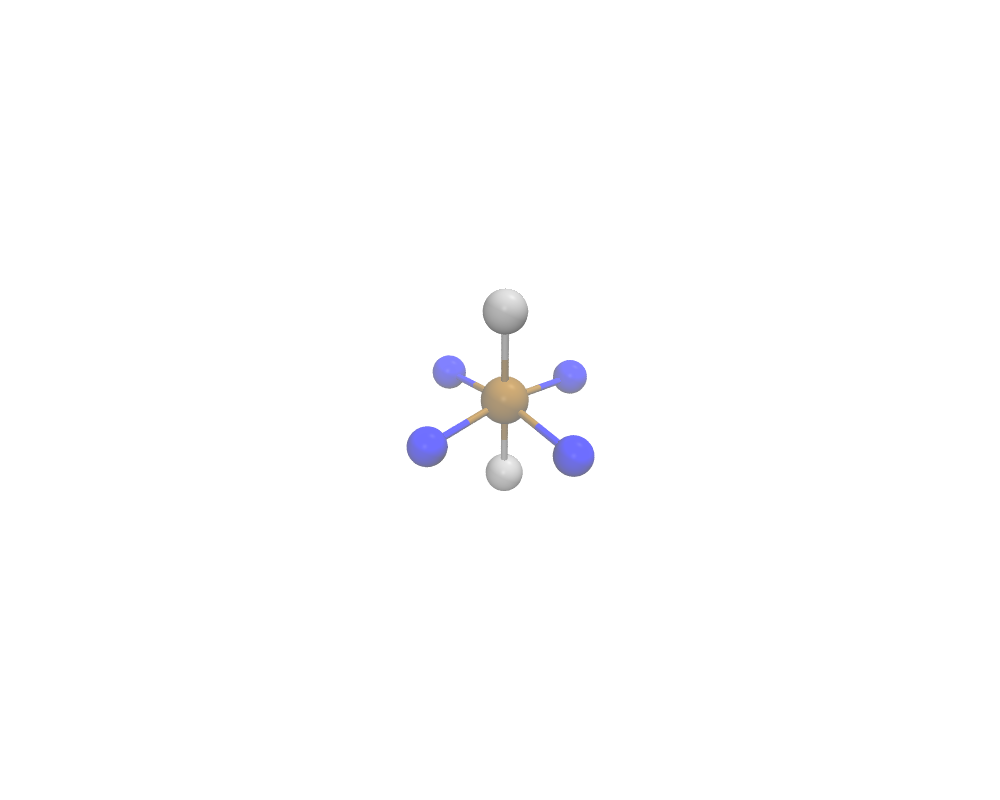
\includegraphics[width=4 cm]{images/local}}};
%\node [orange]  (liex) at (1.5,0.75) {{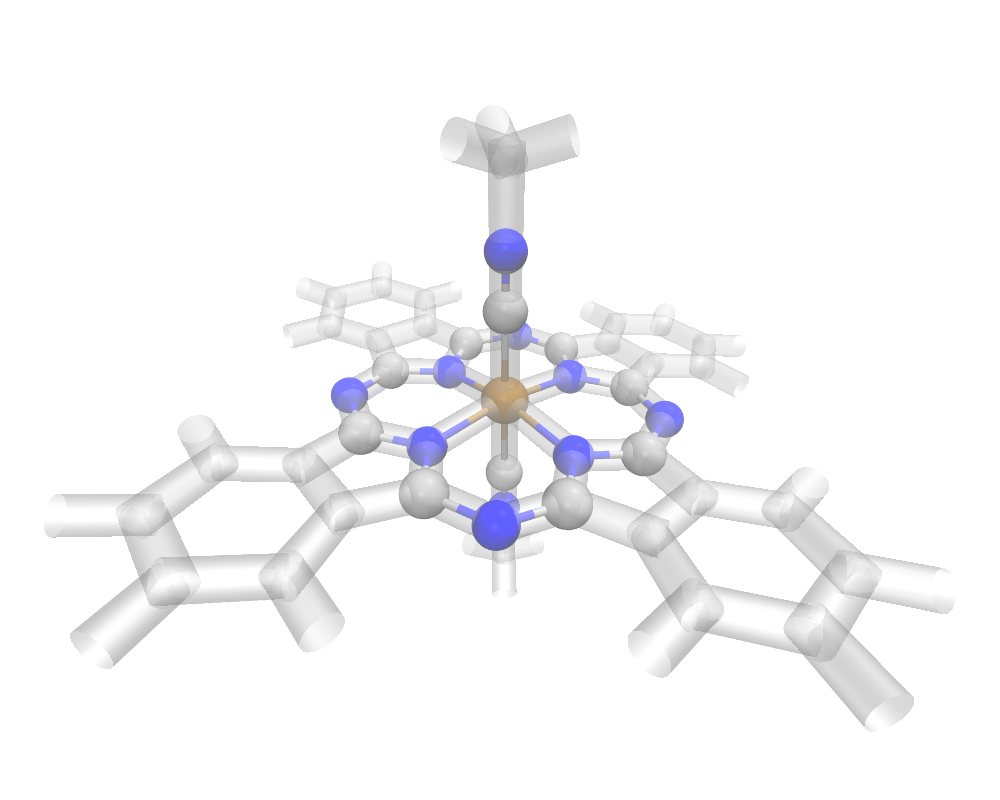
\includegraphics[width=4 cm]{images/partial}}};
%\node [orange]  (liex) at (1.5,0.75) {{\includegraphics[width=4 cm]{images/full}}};



\visible<5->{\node[text width=5cm] at (2.20,0.125){\scriptsize{{Janet, J.P., and Kulik, H.J. \textit{Chem. Sci.}, 2017, 8, 5137-5152.}}};}
\end{tikzpicture}}
\end{center}


